\begin{figure*}[ht]
    \centering
 	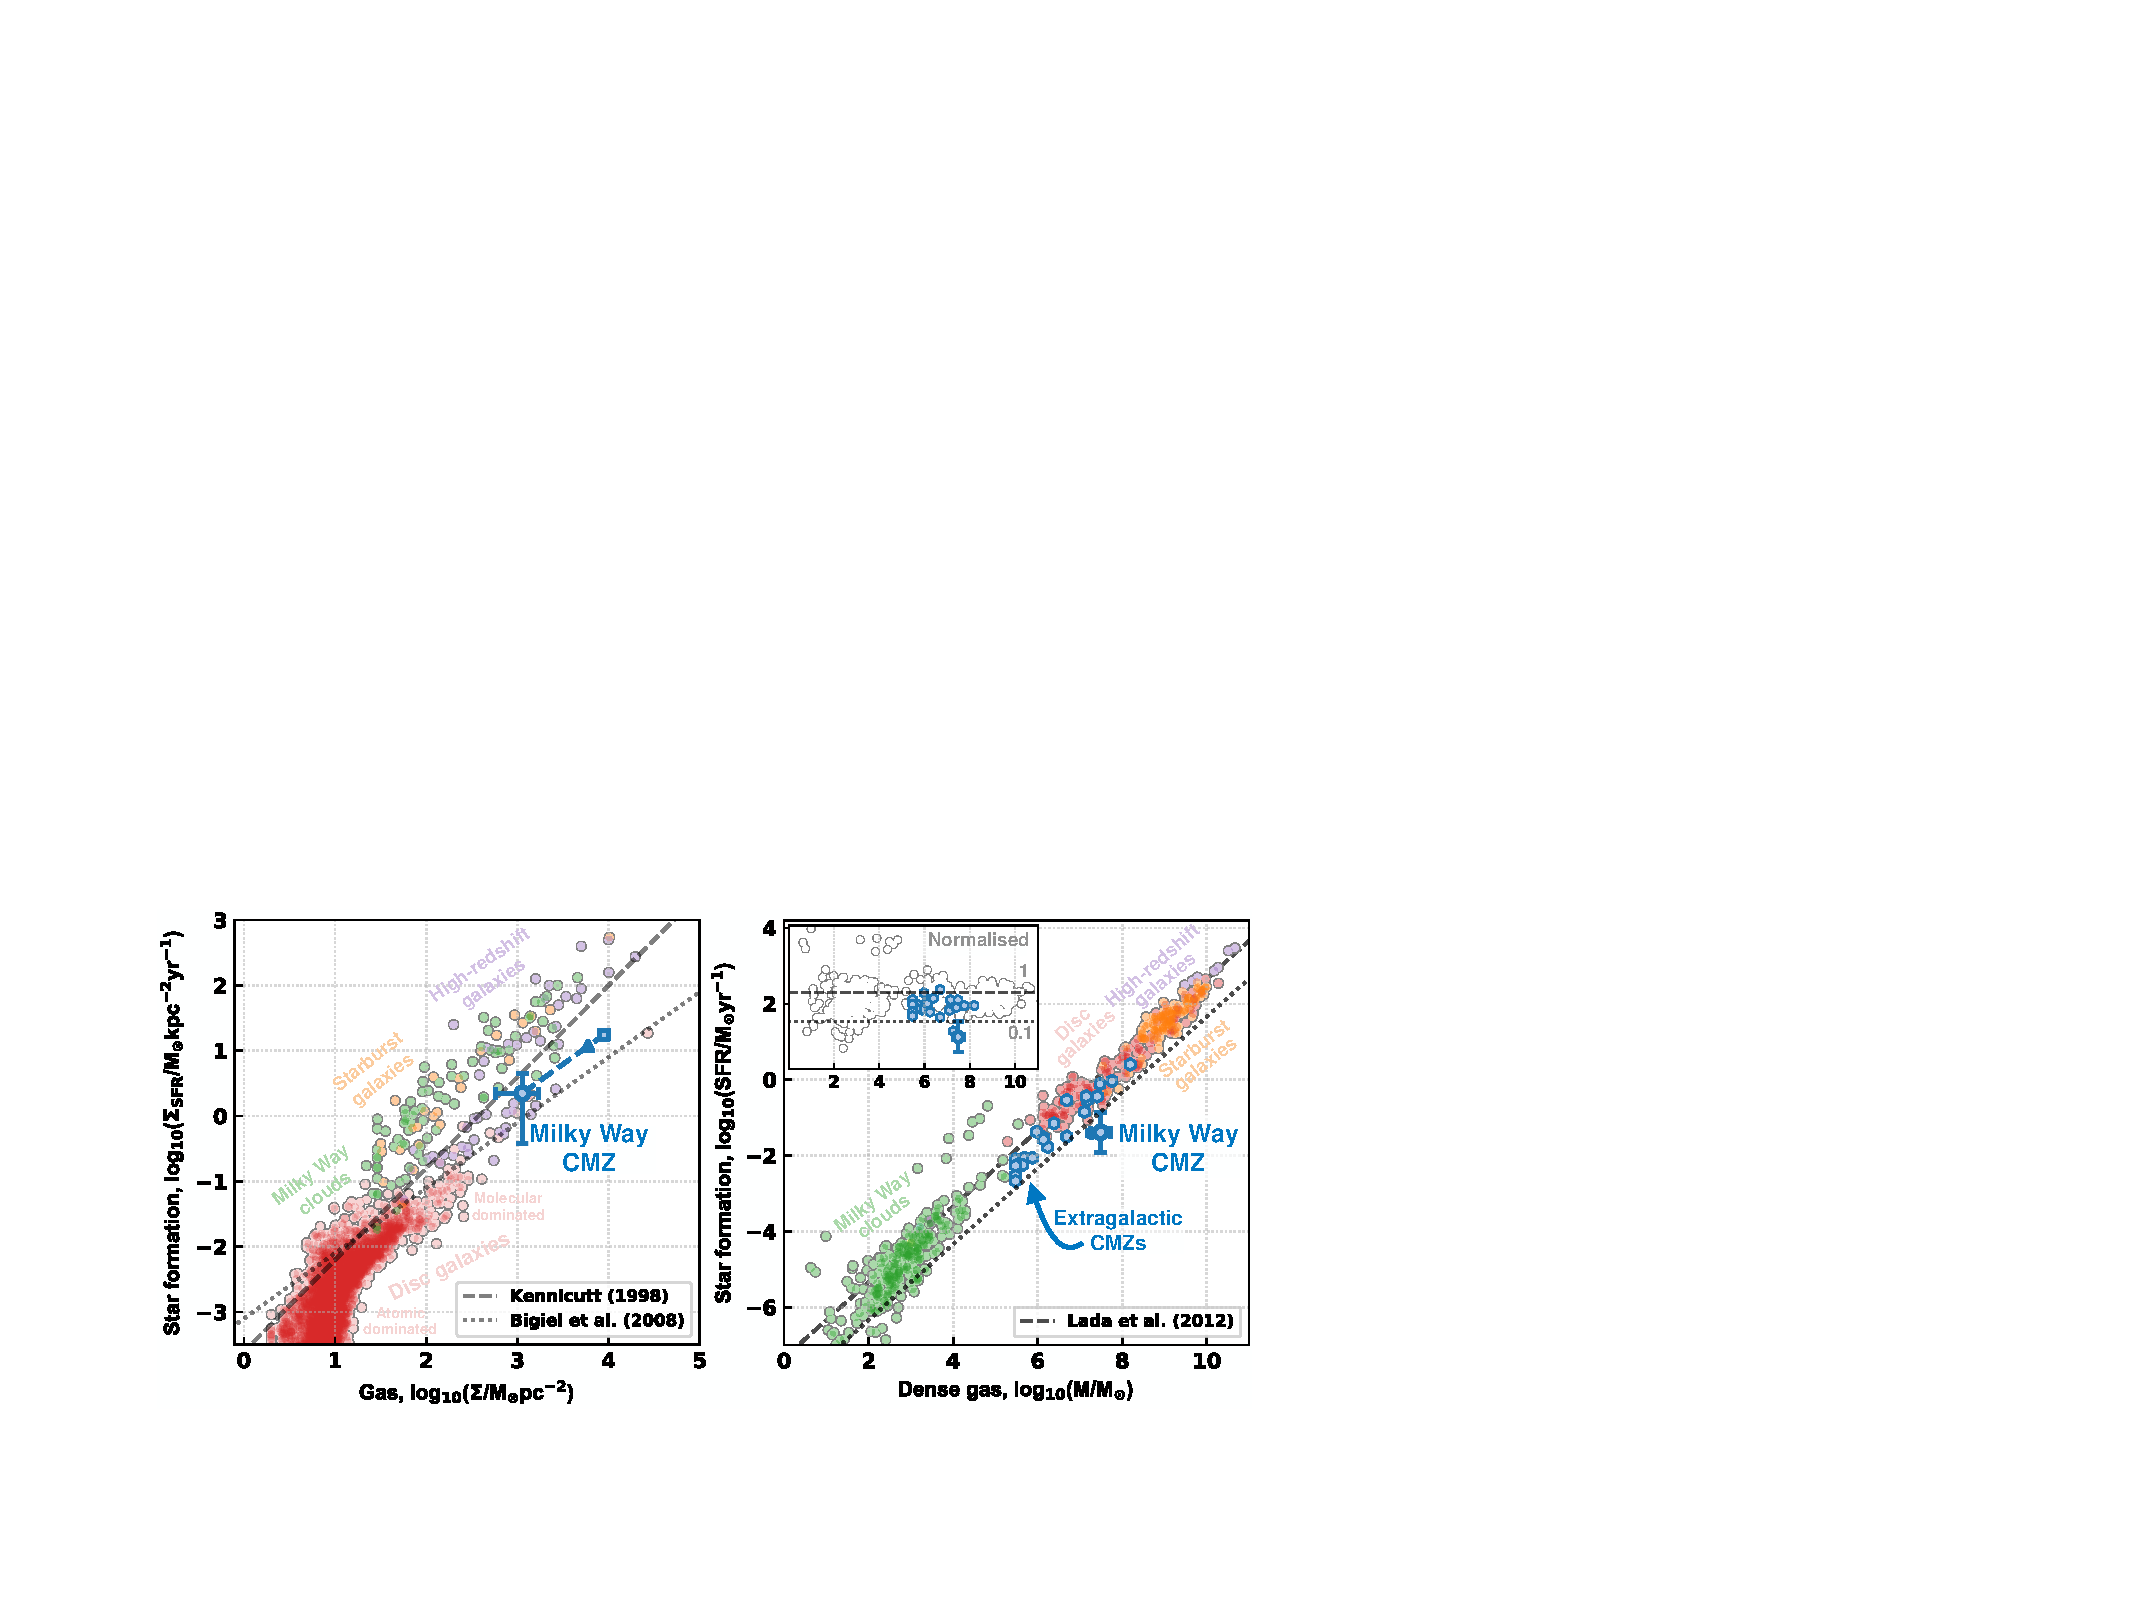
\includegraphics[trim=0 0cm 0 0cm, clip, width=0.85\textwidth]{./figs/sfr_compressed.pdf}
    \caption{The CMZ star-forming properties relative to several commonly used scaling relations. {\em Left:} The SFR surface density ($\Sigma_\mathrm{SFR}$) as a function of the gas surface density ($\Sigma_{\rm gas}$). The CMZ is shown by the large blue circle with error bars, which spans the range of $\Sigma_\mathrm{SFR}$ and $\Sigma_{\rm gas}$ determined in the literature (see Table\,\ref{tab:properties_overview}). This point is determined assuming a face-on disc geometry, whereas the connected points show the results of assuming either face-on ring (triangle) and edge-on geometry (square; see \S\,\ref{subsec:SFR:context}). Shown as grey-outlined coloured points are measurements of systems from the literature (see \citealp{Krumholz2014a} and references therein). Overplotted are the scaling relations from \citet{Kennicutt1998} and \citet{Bigiel2008}. {\em Right:} The relation between the dense molecular gas mass ($M_\mathrm{dense}$) and SFR. The CMZ is shown by the large blue circle with error bars, which span the range of $M_\mathrm{dense}$ and SFR determined in the literature (see Table\,\ref{tab:properties_overview}). Shown as grey-outlined coloured points are the values for systems taken from the literature (see \citealp{Jimenez-Donaire2019} for references). Shown as blue hexagons are extragalactic CMZs (\citealp{Querejeta2019,Jimenez-Donaire2019,Jiang2020,Beslic2021}). The dashed horizontal line shows the scaling relation of \citet{Lada2012}, and the dotted line shows a factor of ten below this relation. {\em Right (inset panel):} The $M_\mathrm{dense}$ and SFR/$M_\mathrm{dense}$, normalised to the \citet{Lada2012} relation.}
    \label{fig:sfr_main}
\end{figure*}
